\documentclass[a4paper, 10pt]{article}
\usepackage{pgf}
\usepackage{eurosym}
\usepackage{graphicx}
\usepackage{wasysym}
\usepackage{hyperref}
\usepackage{listings}
\usepackage{pxfonts}
\usepackage{verbatim}
\usepackage{color}
\usepackage{xcolor}
\usepackage{wrapfig}
\usepackage{enumitem}
\usepackage{booktabs}
\usepackage{tabularx}

\hypersetup{
    bookmarks=true,         % show bookmarks bar?
    unicode=true,          % non-Latin characters in Acrobat’s bookmarks
    pdftoolbar=true,        % show Acrobat’s toolbar?
    pdfmenubar=true,        % show Acrobat’s menu?
    pdffitwindow=true,     % window fit to page when opened
    pdftitle={Assignment 2},    % title
    pdfauthor={Paul Vesey},     % author
    pdfsubject={Construction Project Management},   % subject of the document
    pdfcreator={},   % creator of the document
    pdfproducer={xelatex}, % producer of the document
    pdfkeywords={'Project Management' }, % list of keywords
    pdfnewwindow=true,      % links in new PDF window
    colorlinks=true,       % false: boxed links; true: colored links
    linkcolor=violet,          % color of internal links (change box color with linkbordercolor)
    citecolor=magenta,        % color of links to bibliography
    filecolor=red,      % color of file links
    urlcolor=blue           % color of external links
}

\setlength\parindent{0pt}
\begin{document}

\lstset{language=HTML,
				basicstyle=\small,
				breaklines=true,
        numbers=left,
        numberstyle=\tiny,
        showstringspaces=false,
        aboveskip=-20pt,
        frame=leftline
        }
				
\begin{table}%
	\begin{minipage}{0.4\textwidth}%
			
\includegraphics[width=1\textwidth]{./img/LITlogo.jpg}
	\end{minipage}
	\qquad
	\centering
	\parbox{0.4\textwidth}{
		\begin{large}			
			\begin{tabular}{| r | l |} \hline
				Subject: & \textbf{Construction Project Management}\\
				Course: & \textbf{CPM Special Purpose Award}\\	
				Session: & \textbf{Spring 2020}\\
				Lecturer: & \textbf{Paul Vesey \footnotesize{BEng, MIE, HDip}}\\
				\hline
			\end{tabular}
		\end{large}			
	}
\end{table}
\vspace{0.25cm}	


\begin{flushleft}
\Large\textbf{Assignment 3 (30\%)- Projection and Tracking in Project Libre}\\
\end{flushleft}



\begin{tabularx}{\textwidth}{ |X|X| }
	\hline
	\textbf{Issue Date:} & As stated on Moodle \\
	\hline 
	\textbf{Submission Date:}  & As stated on Moodle  \\
	\hline
\end{tabularx}

\section*{Introduction}

In this assignment you are going to extract data from the project plan provided for the concrete structure shown in figure \ref{fig:building}.  The key deliverables for this project are:

\begin{enumerate}
	\item Excel spreadsheet showing the cost build-up for the project 
	\item Excel line graph showing the cumulative cost build-up for the project 
\end{enumerate}


\begin{figure}[b]
	\centering
	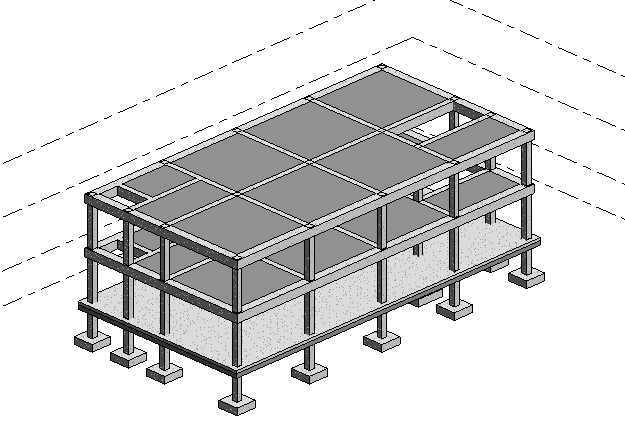
\includegraphics[width=1.0\linewidth]{./img/Building}
	\caption{Concrete Building Structure}
	\label{fig:building}
\end{figure}




\section*{Scenario}

You have been provided with a ProjectLibre file for the construction of the concrete structure shown in figure \ref{fig:building}.  The .pod file contains a simple Gantt chart and resource allocations.  Within the allocations you will also find quantities of concrete added for key features.\\

One objective of the assignment is to extract a cost profile for the construction of the structure at one week intervals.  This information is to be used to create a cost profile using Microsoft Excel.\\

Project Libre lacks some of the functionality that would make this assignment easier.  In order to overcome this shortfall in functionality, it will be necessary to save 'Baselines' within the project and use the 'Status Date' to assist in extracting the correct data.  The data you require can be read from the BCWS column of the Gantt Chart.  You should use the status dates as shown in the table below:


\begin{center}
	\begin{tabular}{ |c|r| }
		\hline
		\textbf{No.} & \textbf{Status Date} \\
		\hline 
		1 & 29 Nov 2019 \\ 
		2 &  6 Dec 2019 \\ 
		3 & 13 Dec 2019\\ 
		4 & 20 Dec 2019\\ 
		5 & 27 Dec 2019\\ 
		6 &  3 Jan 2020\\ 
		7 & 10 Jan 2020\\ 
		8 & 17 Jan 2020\\ 
		9 & 24 Jan 2020\\ 
		10 & 31 Jan 2020\\ 
		\hline
	\end{tabular}
\end{center}

Your second objective is to show an 'Actual Cost' trace for costs incurred on the project up to the 13th of December 2019.  This will be achieved by setting an appropriate precentage completion on the individual activities and reading the data in the 'ACWP' column of the Gantt Chart.  In order to produce the trace, you will need to extract the cumulative ACWP data for 3 weeks.  You are free to overspend or underspend as you see fit in order to produce a suitable trace.


\section*{Submission}
Your completed assignment comprising all computer files are to be zipped into a single file and uploaded to Moodle on or before the date and time indicated.  Key components of the submission are:
\begin{itemize}
	\item Project Libre .pod file
	\item Excel Spreadsheet file
\end{itemize}



\subsection*{Marking Scheme}

\begin{table}[h!]
     \begin{center}
     \begin{tabular}{p{5cm}  p{5cm} }
     \toprule
      \textbf\large{Element} & \textbf\large{Proportion} \\ 
    \cmidrule(r){1-1}\cmidrule(lr){2-2}
      \textbf{Cost Projections} & \textbf{50\%}\\
      \textbf{Cumulative Cost graph} & \textbf{30\%}\\
      \textbf{Actual Cost to 13 Dec 2019} & \textbf{20\%}
      
      \\ \bottomrule
      \end{tabular}
      \label{tbl:markSchemeAsmt3}
      \end{center}
 \end{table}

\end{document}